%pose estimation
\chapter{Activity Recognition}
\label{activityRecognition}

\section{Introduction}

In this section we turn to the problem of recognising and clustering various activities across a range of conditions. We describe an activity as a short sequence of motion, typically undertaken by a person, and captured by either video cameras or a motion capture system. Activity recognition is an important field of study, due to the growing demand for systems that can reliably infer behaviour in a range of settings. There are a wide variety of applications for activity recognition systems. For example in home care scenarios, where robots may be employed to care for the elderly or for the disabled. In home care, the primary consideration is monitoring the status of the patient, to infer, for example, whether they are injured or safe, whether they are cooking or excersing, and most importantly, whether their behaviour appears to be normal.\\

In a similar fashion to previous sections, activity recognition may be used for gaming applications, for example to recognise particular movements that correspond to game commands or to infer the state of the user from their motion. \\

We may also wish to employ activity recognition systems at construction sites. In large workplaces there will be a large number of hazards, for example machinery operating, uncovered holes dug in the ground, and materials swinging through the air as it is transported. This clearly presents significant danger to people as they move about construction sites. It is desirable, therefore, to employ systems that are capable of inferring the trajectory and likely behaviour of people and machinery as they move around. Systems that can identify when someone is walking and discern some information from their gait may also be useful in biometric applications, for instance in security systems, or for use with autonomous vehicles to identify the behaviour of pedestrians.\\


\section{Motion Capture Data}

We are interested in matching time-series signals of various human activities. We are using motion capture data from the Carnegie Mellon dataset, which includes a wide range of activities, for example: walking, running, dancing, climbing over obstacles, swimming motions, getting up off the ground and sweeping motions. The motion capture data contains the angle of each joint over time, as well as the spatial coordinates of a root node. In order to situate our synthetic examples, we first show some examples of real motion capture data. The first two examples, shown in Fig. \ref{getting_up} are of a subject getting up off the ground from a lying position. The second two examples, shown in Fig. \ref{walks} are of a subject walking in a normal fashion. The goal of our algorithm is to measure the similarity between any two motion inputs. We show that our HSIC measure is capable of discriminating between various motions, however we typically require that the motion is first projected into a lower dimensional space. Before we demonstrate our results we will first give an overview of principle component analysis.\\

In many cases our data will lie in a high-dimensional space. Our input motion capture data, for example, has 59 components, six of which describe the position of the root node over time, while the rest describe the angles of various body joints. There is one joint angle per degree of freedom for each particular joint, however not all joints have the full three degrees of freedom. The joint names and the numbers of degrees of freedom are specified in Fig. {mocap image}.\\

\begin{figure}[h]
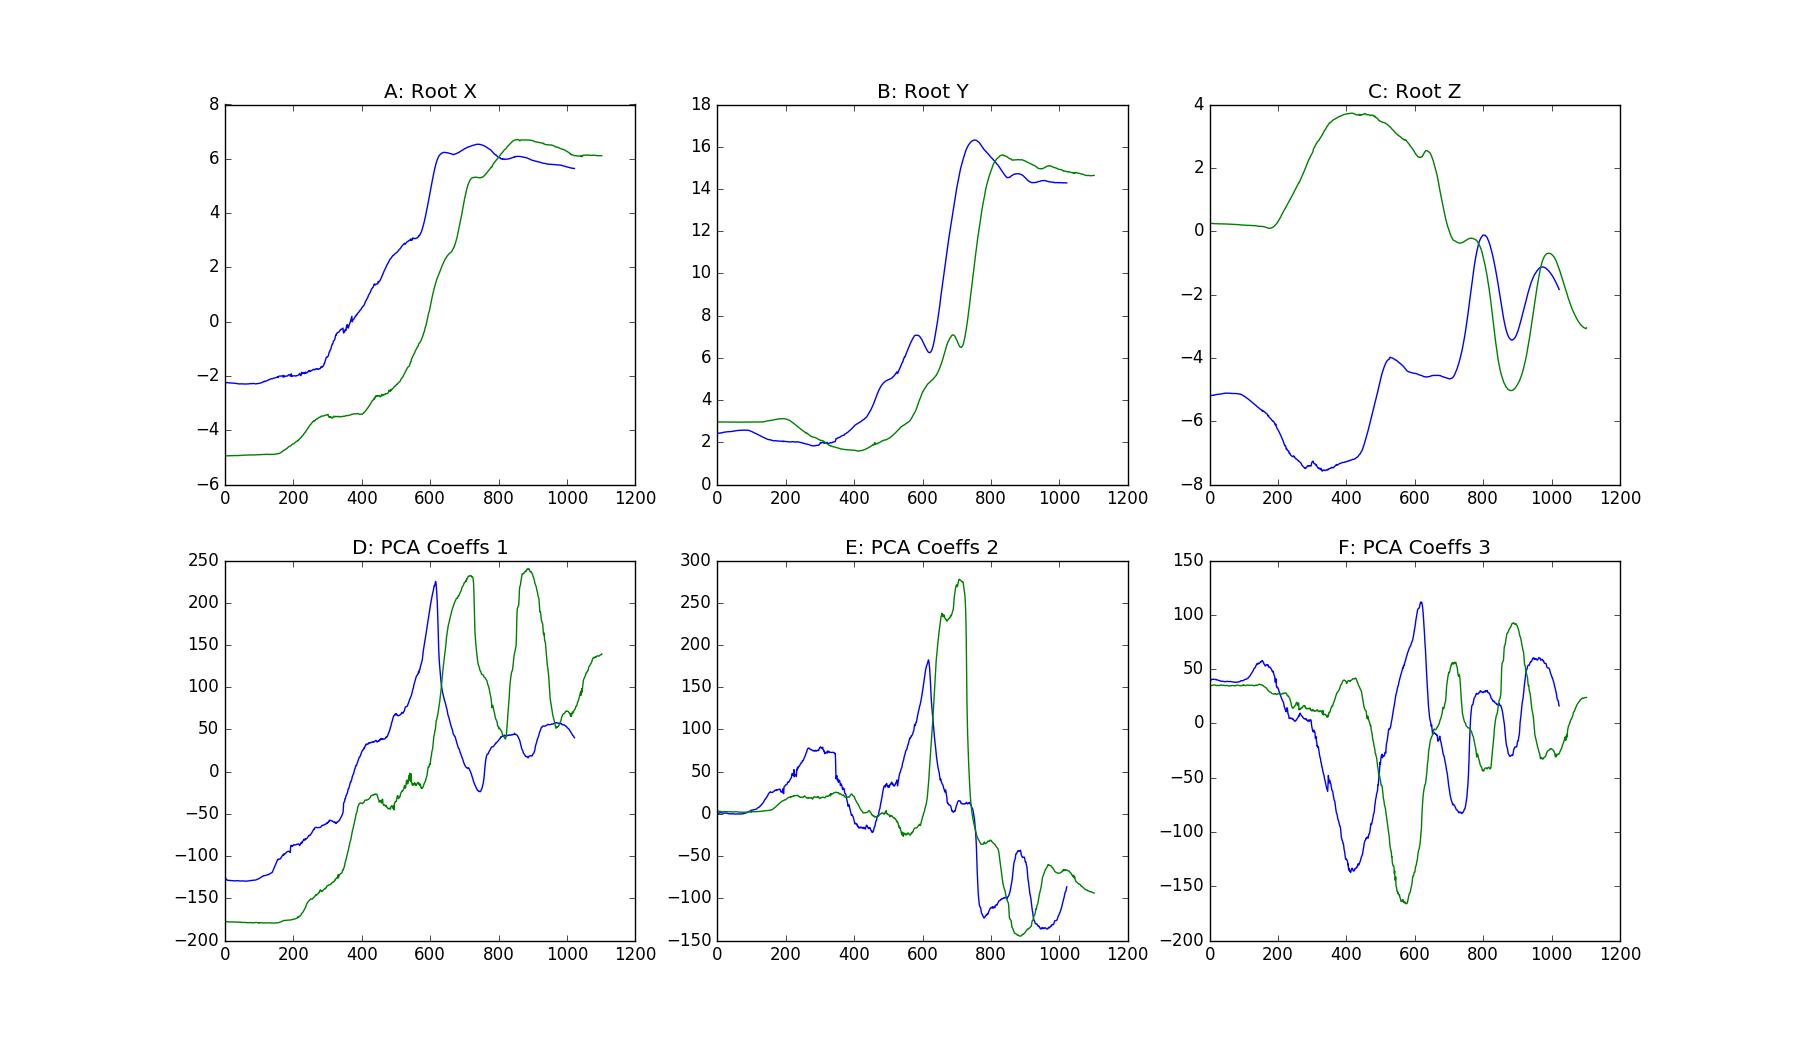
\includegraphics[width=\textwidth]{/home/cshome/j/jcampbell/Desktop/Thesis/Thesis/images/getting_up.png}
\caption{Motion capture data for a subject as they rise from the ground in two 	different examples. The top row shows the position of the root node of the subject while the bottom row shows the data projected according to the PCA basis functions, for each of the first three most significant components. In each of the plots the blue trace is for the first example while the green trace is for the second example. The same subject performed both actions. The two motion examples are 3 and 4 for subject 140 of the CMU Mocap database. \label{getting_up}}
\end{figure}

\begin{figure}[h]
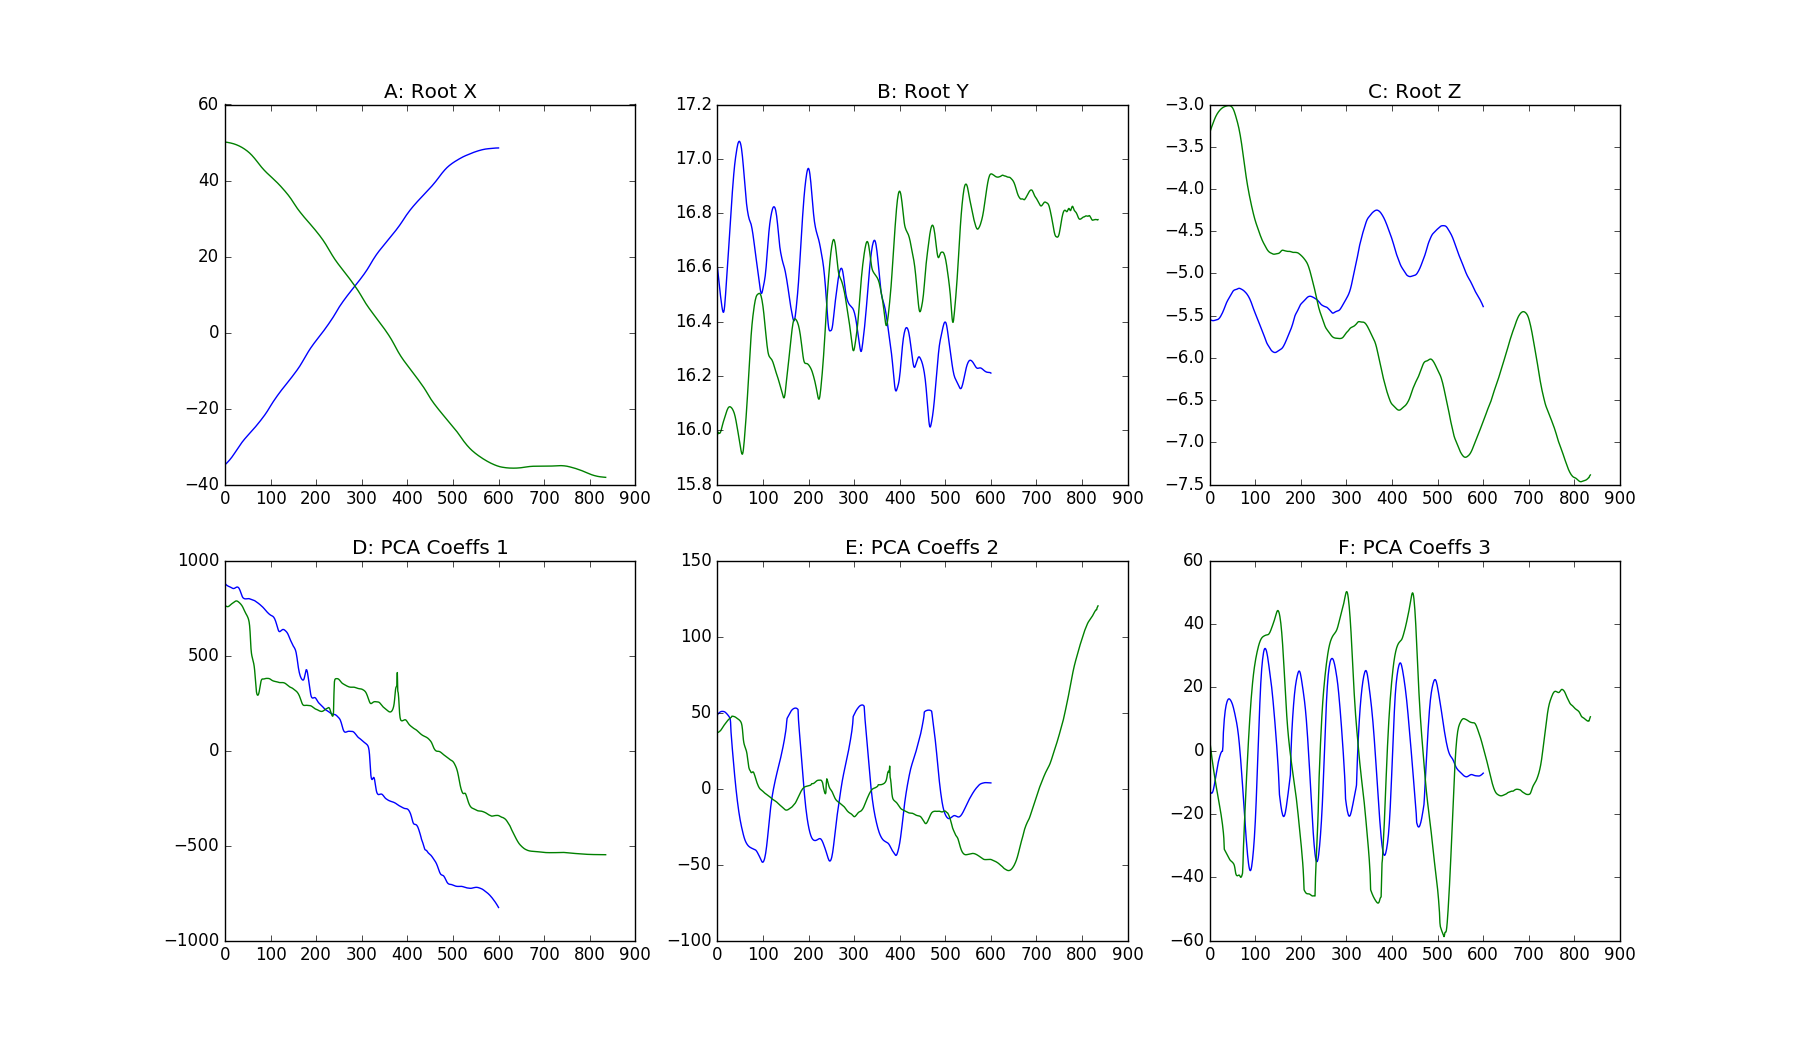
\includegraphics[width=\textwidth]{/home/cshome/j/jcampbell/Desktop/Thesis/Thesis/images/walks.png}
\caption{Motion capture data for a subject as they walk in two different examples. In both cases the subject walked for a short period in one direction and then turned and walked back. The top row shows the position of the root node of the subject while the bottom row shows the data projected according to the PCA basis functions, for each of the first three most significant components. In each of the plots the blue trace is for the first example while the green trace is for the second example. The same subject performed both actions. The two motion examples are 21 and 22 for subject 136 of the CMU Mocap database. \label{walks}}
\end{figure}

\subsection{Principle Component Analysis}

Principle component analysis (PCA) is a widely used method for computing a low dimensional representation of data. Given an $n\:\:\text{x}\:\:m$ data matrix $X$, PCA finds a linear transformation to a new set of coordinate axes such that the variance along each of the new axes is maximised. Typically singular value decomposition (SVD) is used to find this transformation. The PCA transform using SVD performs a factorisation of the data matrix according to

\begin{equation}
X = U \Sigma V^{T} 
\end{equation}

\noindent where $U$ and $V$ are the left and right singular vector matrices of size $n\:\:\text{x}\:\:n$ and $m\:\:\text{x}\:\:m$ respectively. The matrix $\Sigma$ is an $n\:\:\text{x}\:\:n$ diagonal matrix containing the $n$ singular values of $X$. The vectors of $V$ are eigenvectors of the covariance matrix $X X^{T}$ and represent the principle components of the transformed data. We transformed data matrix is found by projecting the original data matrix into the space defined by the PCA axes according to

\begin{equation}
Y = V X. 
\label{PCA_compute}
\end{equation}

This method, however, only works efficiently in cases where the dimensionality of each sample is much lower than the number of samples available, i.e. when $n > p$. This is because the covariance matrix $X X^{T}$ becomes very large. \\

It is often the case where the dimensionality of our samples is much greater than the number of samples available. We will see in later sections that this is the case for temporal synchronisation of videos. If we represent each frame of a video as a single vector then the dimensionality of each sample is equal to the number of pixels in the image. If our video is only 100 - 200 frames long, then we clearly have $p >> n$. In this situation we turn to an alternative method for estimating the principle components, as defined by reference. \\

Since the number of samples is low we can efficiently compute the alternative covariance matrix $X^{T} X$ which is of size $n\:\:\text{x}\:\:n$. We then compute the eigenvalues and eigenvectors of this covariance matrix. The matrix $V$ is formed by stacking the eigenvectors in columns according to the size of the corresponding eigenvalues and can then be used as in Eq. \ref{PCA_compute}.\\






















\section{Synthetic Function Matching with HSIC}

The principle contribution of this section is to demonstrate that our HSIC based measure provides a robust measure of the similarity between two arbitrary time-series signals. We demonstrate this capability with a series of examples on synthetic data. As a further proof of concept we also demonstrate that our measure could be used to re-construct a signal from data, in cases where Fourier based methods are not suitable. \\

We saw in Figs \ref{getting_up} and \ref{walks} that our input is a multi-dimensional time-series signal. The top rows of each of these figures are raw input data, while the bottom rows are the PCA transformed data. In each plot we have traced a single parameter from each of two motions. Our input is given by the variables $X = \{x_0, x_1, ..., x_n\}$ and $Y = \{y_0, y_1, ..., y_n\}$, where each of the $n$ samples $x_i$ and $y_i$ are vectors of length $m$. Each element of $x_i$ and $y_i$ gives the value of a single parameter at a single point in time. As usual we have that $\text{HSIC}(X, Y) = \frac{1}{n^2}\textbf{KHLH}$ where $\textbf{H}$ is a centering matrix and $\textbf{K}$ and $\textbf{L}$ are Gram matrices defined on $X$ an $Y$ respectively. As before, our kernel matrix is defined as

\begin{equation}
\textbf{K}_{i,j} = k(x_i,y_j) = \exp^{-((x_i-y_j)\Sigma(x_i-y_j)^T)}
\end{equation}

\noindent where $\Sigma$ is a covariance matrix.\\

Before we begin a discussion of further experiments we first introduce our normalised version of the HSIC, which we term NHSIC. The NHSIC is defined as 

\begin{equation}
\text{NHSIC}(X,Y) = \frac{\text{HSIC}(X,Y)}{\sqrt{\text{HSIC}(X,X)\text{HSIC}(Y,Y)}}
\end{equation}

\noindent and is necessary because, as we will see, we need to vary the choice of (co)-variance for any choice of $X$ and $Y$. We therefore need to scale the HSIC value in order to be able to compare any two results. This will be elaborated further below. \\

In previous works a number of authors have used the median of the data values as the variance in the kernel function. We show instead that it is better to estimate the (co)-variance from the data. This produces much more stable results than the median value, which is important if we are using the NHSIC as an energy measure in an optimisation schema. In Fig. \ref{var_med} we show how the choice of variance affects the HSIC between a fixed signal and a signal with a varying amplitude. In the left plot we can see that the NHSIC varies smoothly with changes in the amplitude of the test signal, while in the right plot the NHSIC results are noisy and contain a significant number of local minima.\\

\begin{figure}[h]
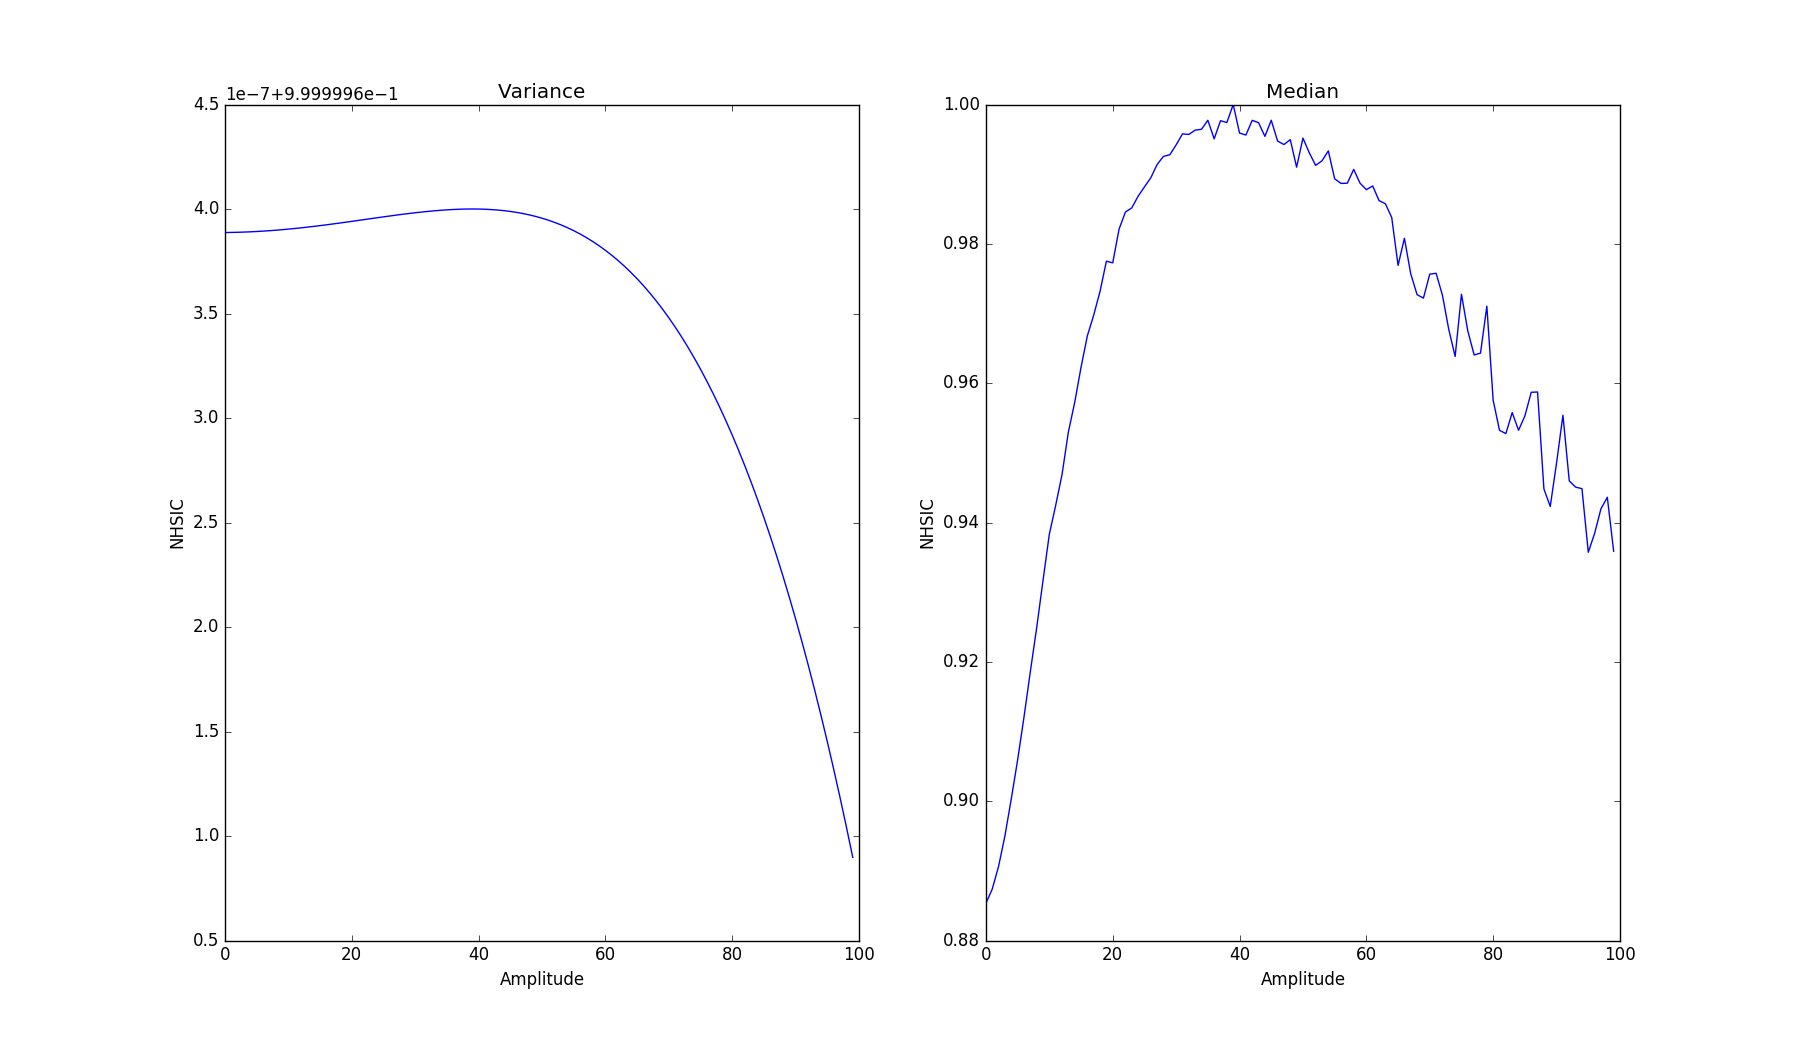
\includegraphics[width=\textwidth]{/home/cshome/j/jcampbell/Desktop/Thesis/Thesis/images/var_med.png}
\caption{NHSIC results using the variance estimated from data (left plot) and the median of the values (right plot) to measure the similarity between a signal with a fixed amplitude and another with a varying amplitude. It is difficult to see in the left plot however the maximum value 9at index 39) is correct, as is that for the right plot.  \label{var_med}}
\end{figure}

One of the consequences of performing computations on sine waves is that the variance of the signal increases quadratically with linear increases in the amplitude. This effect can be seen in Fig. \ref{amp_var} which demonstrates the changes in variance as the amplitude of a sine wave increases. If we were to choose a fixed value for the (co)-variance in the kernel function, then we would effectively be restricting the domain of the kernel function given the variance of the input signal. At first glance this would seem fine, as it is our goal to discover differences in two signals, which will clearly be uncovered if our kernel function treats signals with different variances differently. The problem, however, is that as the magnitude of a sine wave approaches infinity, the HSIC will approach a value of one. This means that a signal with a large amplitude is deemed more similar to a reference signal than the reference signal with itself. If we are given the three functions: $f_1(x) = 0.9\sin(x)$, $f_2(x) = 0.25\sin(x)$, and $f_3(x) = 2.5\sin(x)$, with the goal of asking which of $f_1$, $f_1$, or $f_1$ is most similar to $f_{\text{ref}}(x) = \sin(x)$, then we would be given $f_3$ as the closest match. Notably, if the (co)-variance of the kernel function is fixed, then we would have that $\text{HSIC}(f_{\text{ref}}, f_3) > \text{HSIC}(f_{\text{ref}}, f_{\text{ref}})$. Thankfully the solution to this problem is very simple: we require only that the variance of the kernel function be estimated independently for any HSIC computation. As mentioned previously, however, this means that we must also normalise the resulting HSIC value.  \\

In Figs. \ref{fixed_var_no_norm}, \ref{floating_var_no_norm}, \ref{fixed_var_normalisation}, and \ref{floating_var_normalisation} we show the effect of computing the HSIC between two sine waves, one with varying amplitude and frequency, under a number of different conditions. In all four of these experiments the same test sine wave was used. In Figs. \ref{fixed_var_no_norm} and \ref{floating_var_no_norm} the incorrect result is returned, while in Fig. \ref{fixed_var_normalisation} the correct result is returned, however it is less distinct than the (correct) results in Fig. \ref{floating_var_normalisation}. It is difficult to see in these examples, however the correct frequency is obtained for almost all magnitudes. In Fig. \ref{freq} we can see that at the correct magnitude the correct frequency is clearly found by our algorithm. 



\begin{figure}[h]
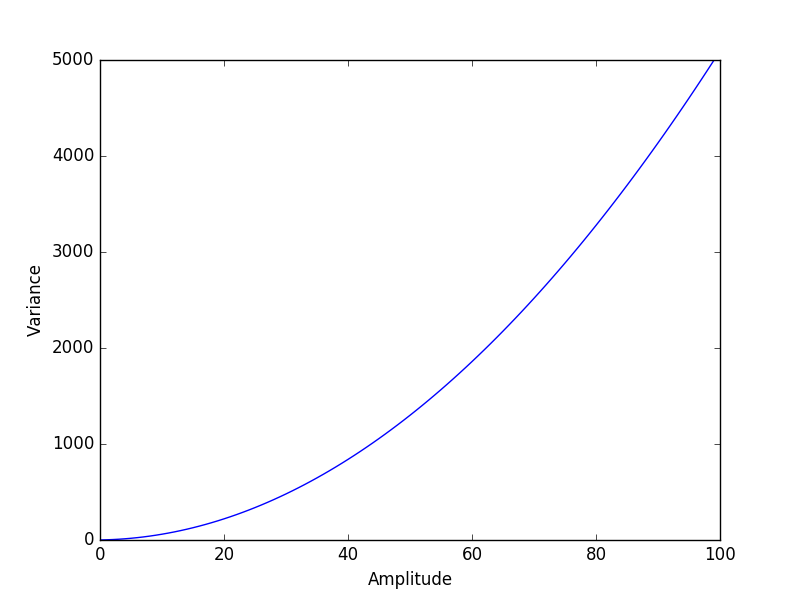
\includegraphics[width=\textwidth]{/home/cshome/j/jcampbell/Desktop/Thesis/Thesis/images/amp_var.png}
\caption{Variance of a sine wave as the magnitude is linearly increased.\label{amp_var}}
\end{figure}

\begin{figure}[h]
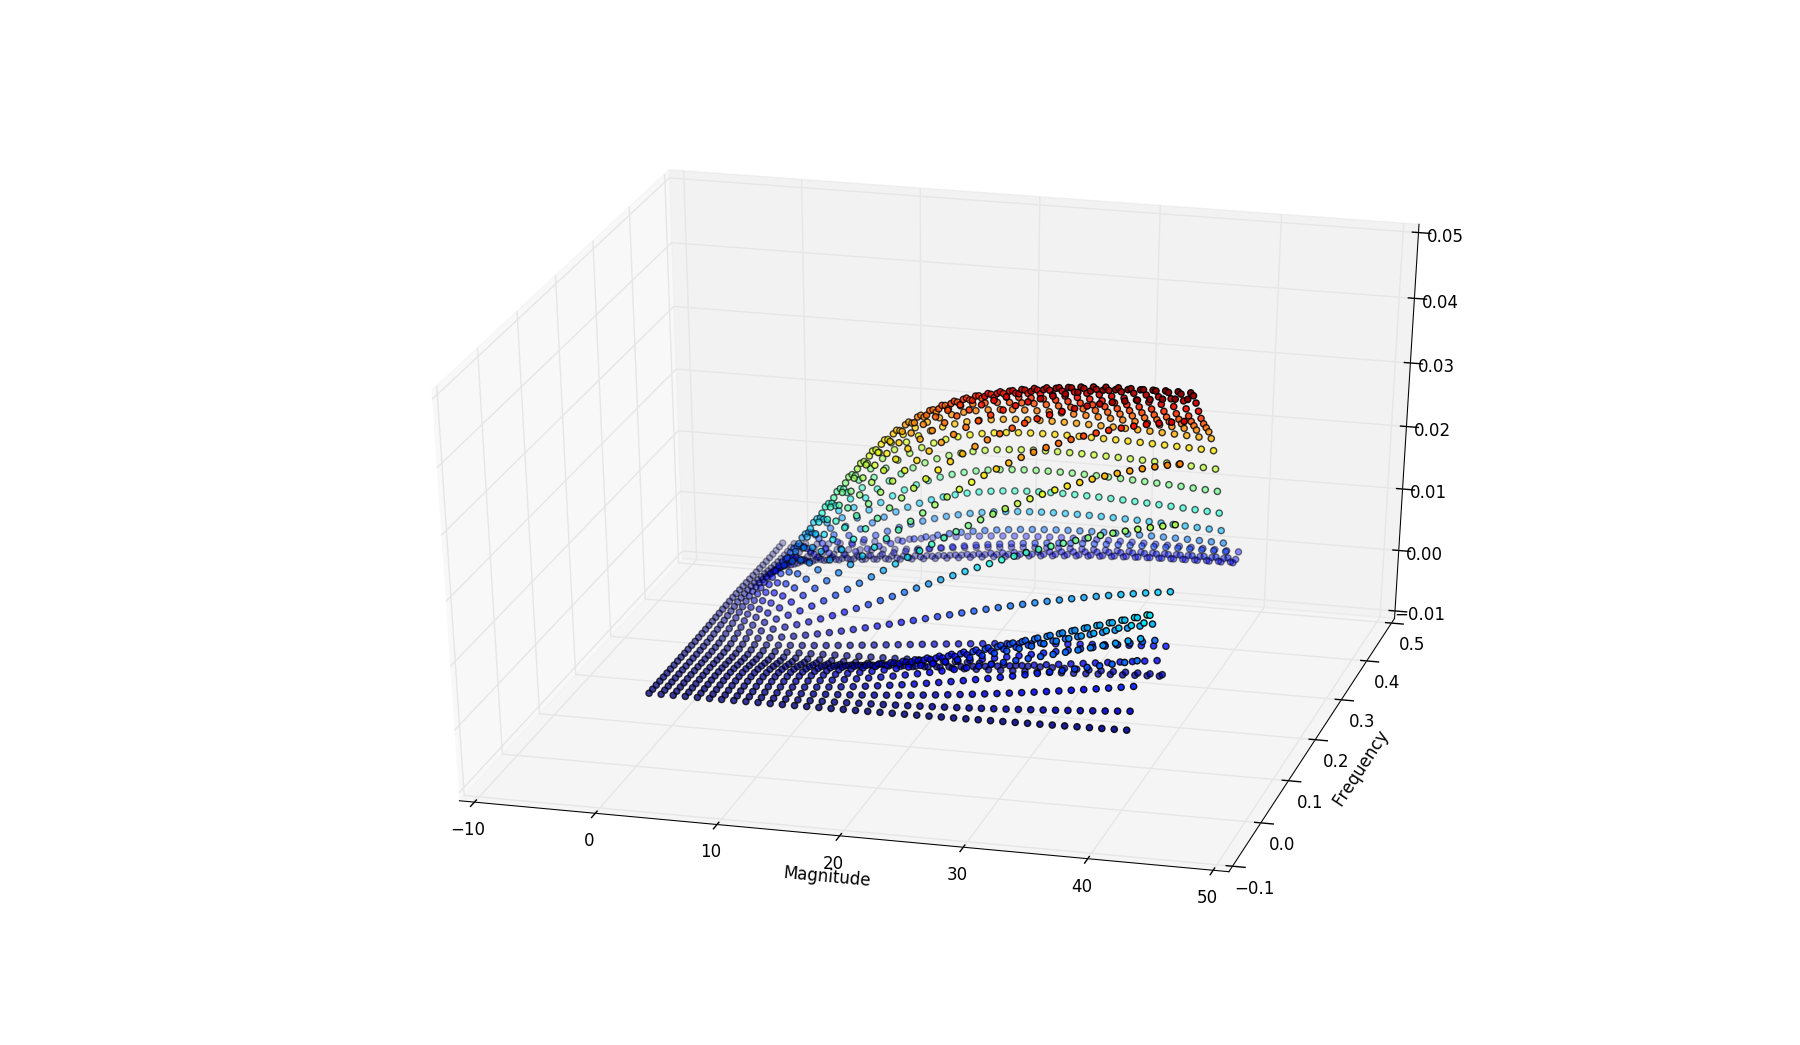
\includegraphics[width=\textwidth]{/home/cshome/j/jcampbell/Desktop/Thesis/Thesis/images/fixed_var_no_norm.png}
\caption{Variance computed from all possible examples, with no normalisation of the HSIC.\label{fixed_var_no_norm}}
\end{figure}

\begin{figure}[h]
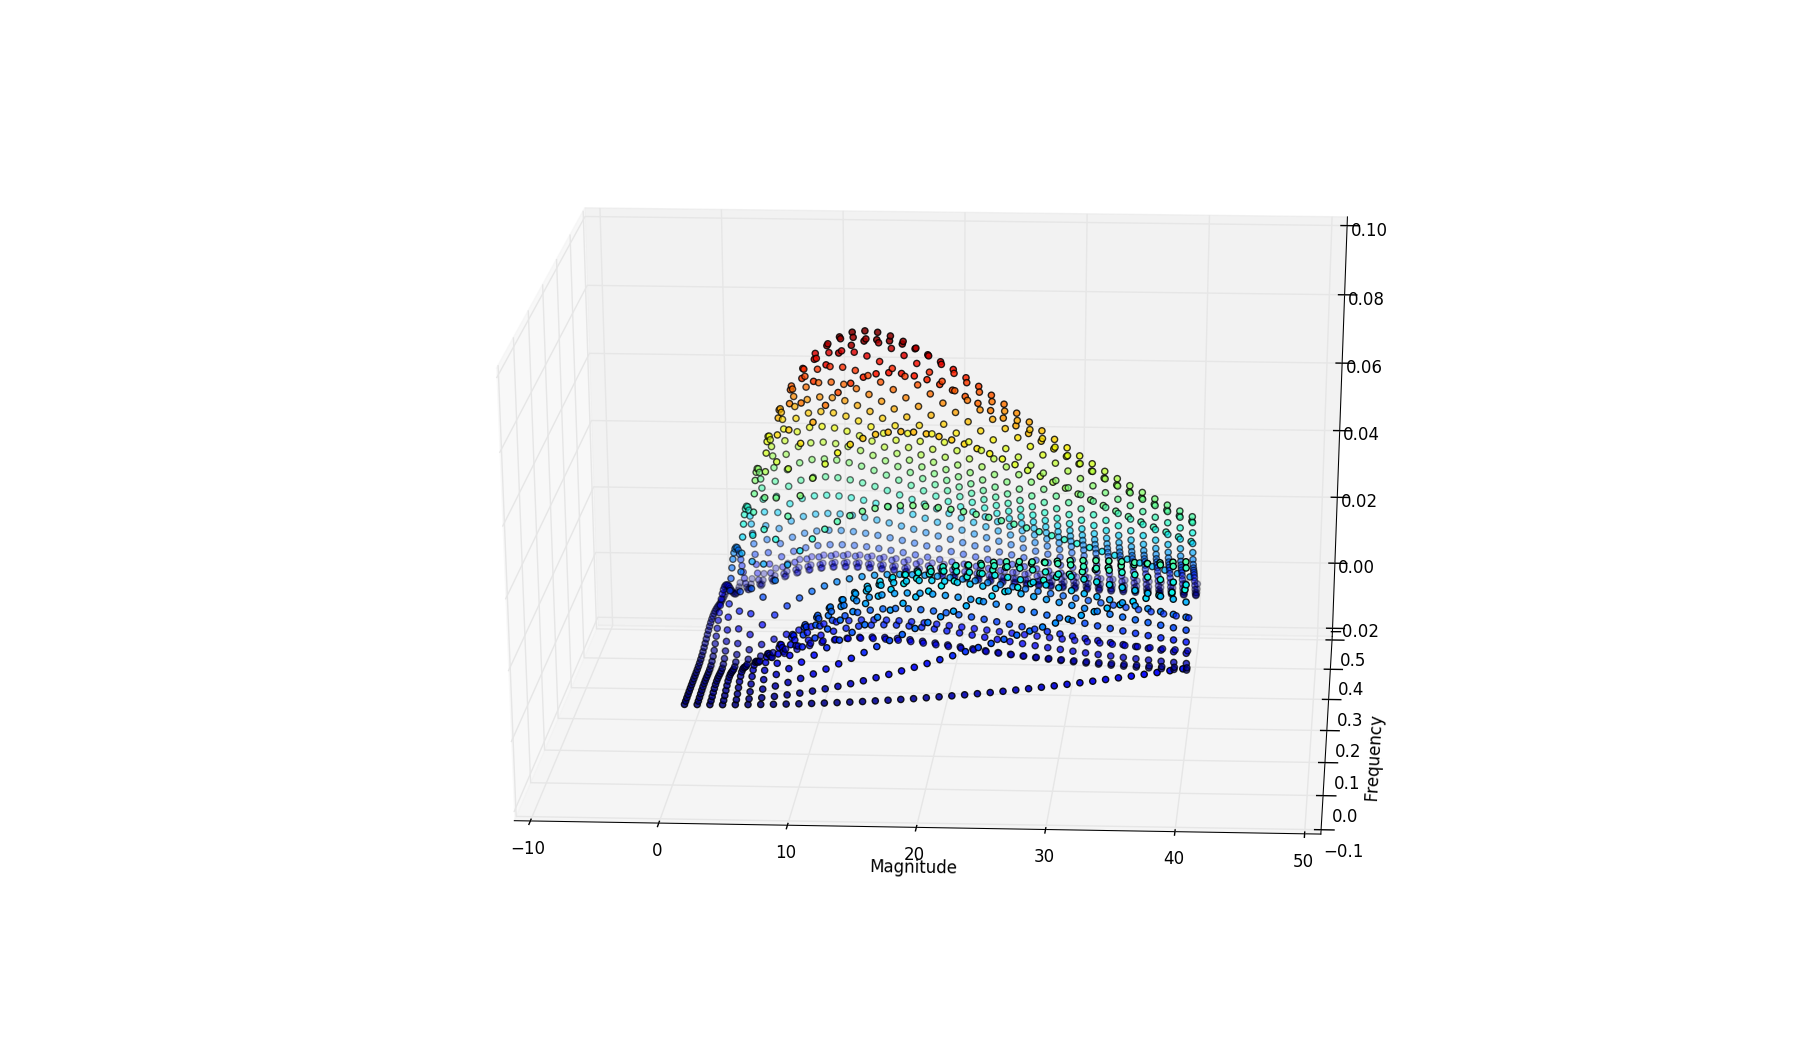
\includegraphics[width=\textwidth]{/home/cshome/j/jcampbell/Desktop/Thesis/Thesis/images/floating_var_no_norm.png}
\caption{Variance computed independently for every test example, with no normalisation of the HSIC.\label{floating_var_no_norm}}
\end{figure}

\begin{figure}[h]
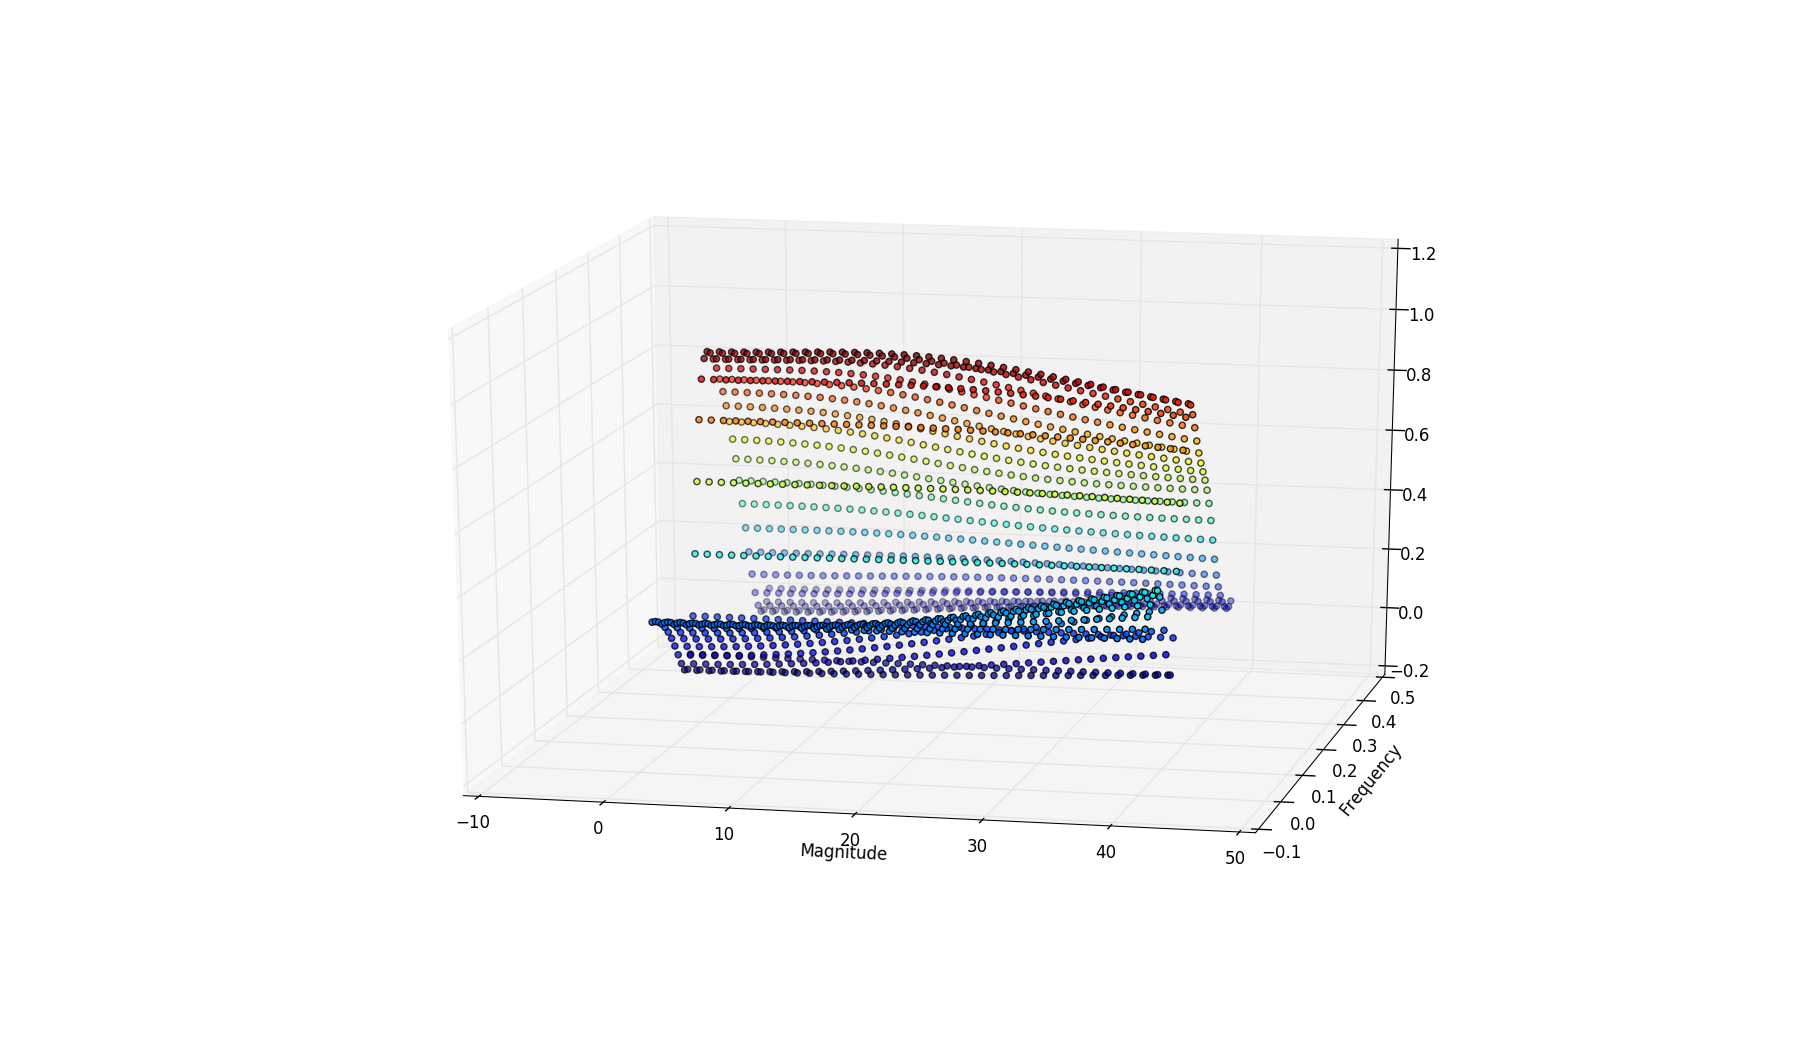
\includegraphics[width=\textwidth]{/home/cshome/j/jcampbell/Desktop/Thesis/Thesis/images/fixed_var_normalisation.png}
\caption{Variance computed from all possible examples, with normalisation of the HSIC.\label{fixed_var_normalisation}}
\end{figure}

\begin{figure}[h]
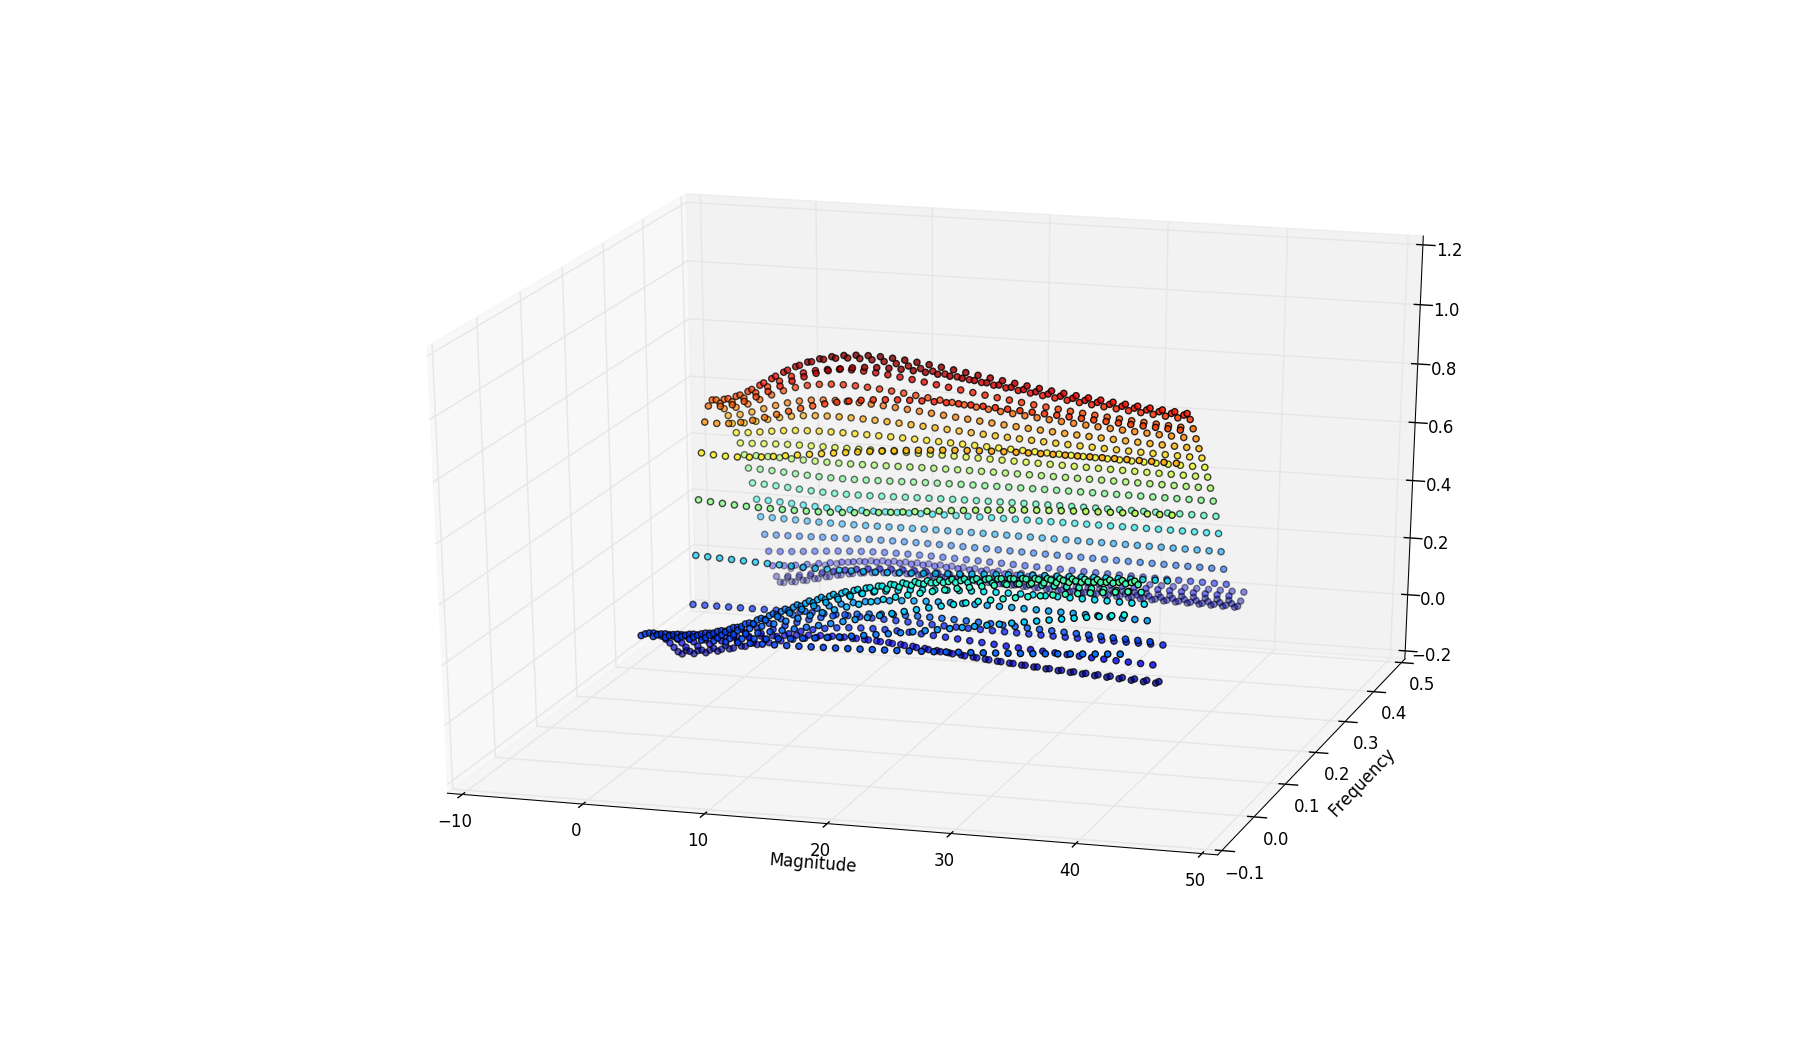
\includegraphics[width=\textwidth]{/home/cshome/j/jcampbell/Desktop/Thesis/Thesis/images/floating_var_normalisation.png}
\caption{\label{floating_var_normalisation}}
\end{figure}

\begin{figure}[h]
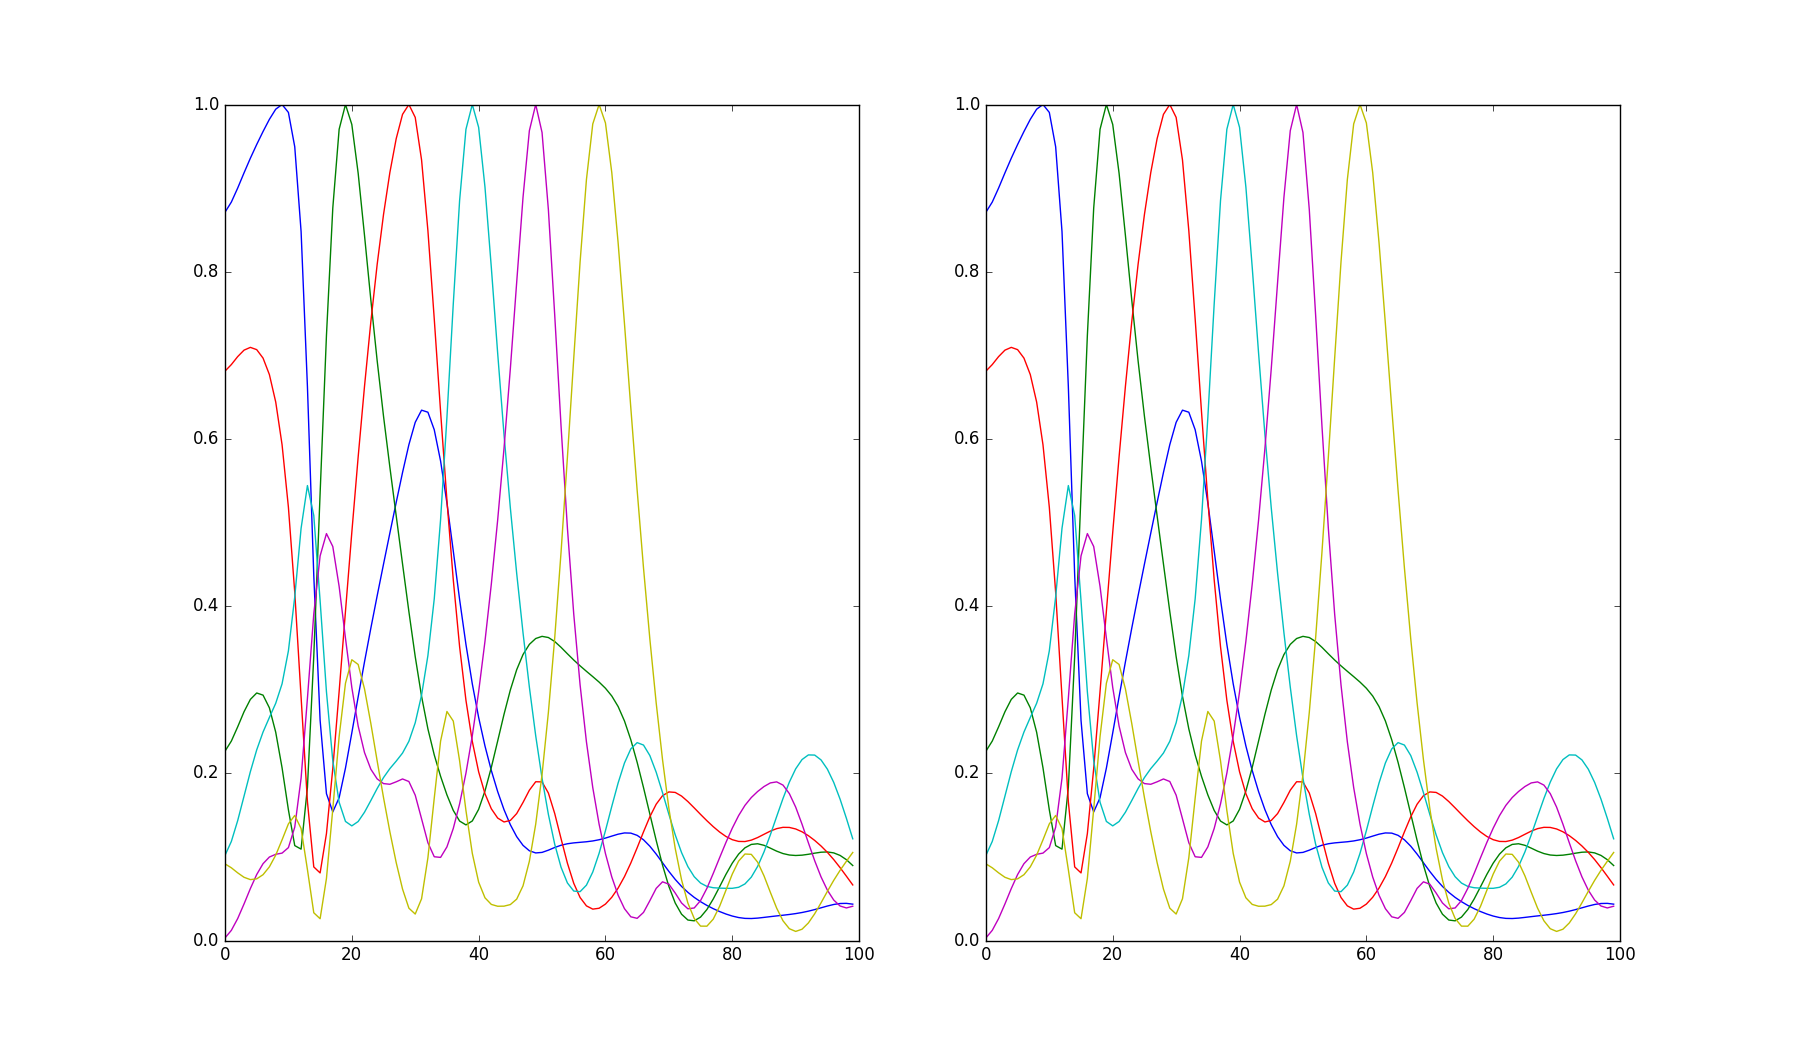
\includegraphics[width=\textwidth]{/home/cshome/j/jcampbell/Desktop/Thesis/Thesis/images/freq.png}
\caption{\label{freq}}
\end{figure}

\begin{figure}[h]
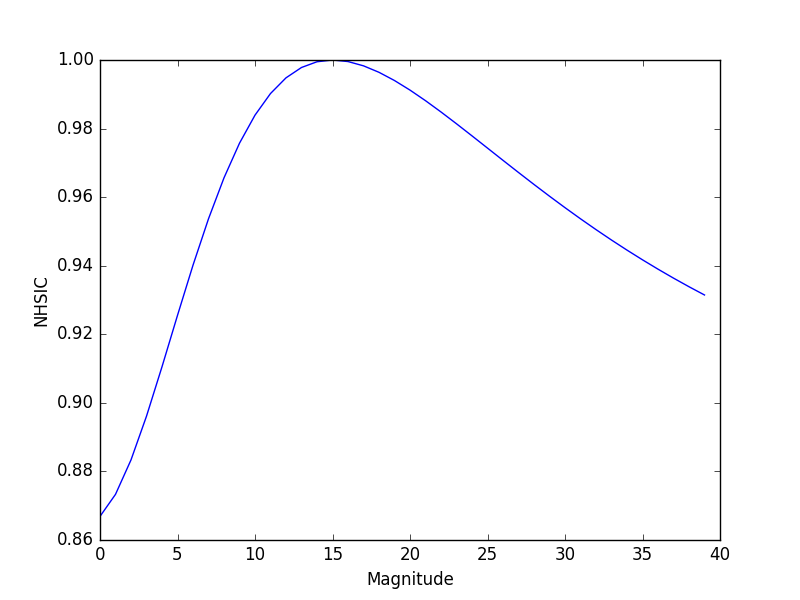
\includegraphics[width=\textwidth]{/home/cshome/j/jcampbell/Desktop/Thesis/Thesis/images/magnitude.png}
\caption{\label{magnitude}}
\end{figure}


\section{Temporal Synchronisation}

There are often times when two vides of an activity will not be temporally aligned, for example in film making. In the film industry the term 'shot' is used to denote a short sequence of continuous activity which is not broken by a cut, typically on the order of 1000 frames. It is common for multiple cameras to record each shot, as well as infrared cameras if motion capture technology is being employed. Motion capture systems typically contain their own dedicated hardware temporal synchronisation frameworks, while an additional hardware synchronisation system is employed for the remaining cameras. Hardware synchronisation methods are occasionally used for filming outdoors, however they are often costly and require time to setup for each shoot. Hardware synchronisation methods are therefore inaccessible for amateur cinematographers, and for unplanned, ad hoc recording scenarios. In these situations it is therefore highly likely that the activity recorded from each camera will not be synchronised in time. Furthermore, even if hardware synchronisation has been used, once a shot has been captured it will often be sent to an editorial team, who may perform alterations to the shot which renders the timestamps incorrect. The original and the modified shots will therefore require manual synchronisation to align them again. Manual synchronisation is typically performed by searching for high frequency events such as footfalls, eyeblinks, or when any two items connect. This obviously introduces problems when there is very little scene activity, or when there are no high frequency components. This could occur in tracking shots that produce a sweeping motion, or for shots in which any activity is very smooth, for example a car driving along a street. \\

It is vitally important that multiple views of a shot are aligned in time. In live action films it is critical to know when to be able to switch between views, while in films that contain visual effects elements the multiple views are used as input to motion reconstruction pipelines, stereo reconstruction pipelines, and as raw input for artists manually creating creatures and scenes. \\

\section{Activity Clustering}
